%%%%%%%%%%%%%%%%%%%%%%%%%%%%%%%%%%%%%%%%%%%%%%%%%%%%%%%%%%%%%%%%%%%%%%%%%%%%%%%
% SC26 UTEP-style research poster — editable baposter source
%%%%%%%%%%%%%%%%%%%%%%%%%%%%%%%%%%%%%%%%%%%%%%%%%%%%%%%%%%%%%%%%%%%%%%%%%%%%%%%
\documentclass[
landscape,
final,
paperwidth=48in,
paperheight=36in,
fontscale=0.30
]{baposter}

\usepackage[T1]{fontenc}
\usepackage[utf8]{inputenc}
\usepackage{lmodern}
\usepackage{graphicx}
\usepackage{amsmath,amssymb}
\usepackage{booktabs}
\usepackage{enumitem}
\usepackage{ragged2e}
\usepackage{tikz}
\usetikzlibrary{arrows.meta,positioning,shapes.geometric}
\newcommand{\PosterTitle}{Earth's Core: Exploring Iron Allotropes under Extreme Conditions through First-Principles Simulations and Graph-Kernel-Based Machine Learning}
\newcommand{\PosterAuthors}{Diego Ju\'arez}
\newcommand{\PosterAffiliation}{Department of Physics, The University of Texas at El Paso}
\newcommand{\PosterEmail}{IronCoreMD Project \textbar{} Email to be added before submission}


\definecolor{uteporange}{RGB}{245,128,37}
\definecolor{utepdark}{RGB}{86,43,18}
\definecolor{utepsoft}{RGB}{255,247,239}
\definecolor{utepblue}{RGB}{0,78,122}
\definecolor{utepgray}{RGB}{64,64,64}
\definecolor{resultgreen}{RGB}{34,120,82}

\setlength{\columnsep}{1.0em}
\setlength{\columnseprule}{0mm}
\setlist[itemize]{leftmargin=1.15em,itemsep=0.18em,topsep=0.20em,parsep=0pt}
\newcommand{\tightlist}{\setlength{\itemsep}{0.12em}\setlength{\parskip}{0pt}}
\newcommand{\metric}[2]{%
  \fcolorbox{uteporange}{utepsoft}{\parbox[c][2.15em][c]{0.29\linewidth}{\centering
  \textcolor{utepdark}{\bfseries\Large #1}\\[-0.2em]\scriptsize #2}}}

\begin{document}
\begin{poster}
{
  headerborder=closed,
  colspacing=0.82em,
  bgColorOne=white,
  bgColorTwo=white,
  borderColor=uteporange,
  headerColorOne=utepdark,
  headerColorTwo=uteporange,
  headerFontColor=white,
  boxColorOne=white,
  columns=3,
  textborder=roundedleft,
  eyecatcher=true,
  headerheight=0.115\textheight,
  headershape=roundedright,
  headerfont=\Large\bfseries,
  linewidth=2pt
}
% Official UTEP logo supplied in the poster figures directory.
{\IfFileExists{figures/utep+loog.png}{
\includegraphics[height=7.5em]{figures/utep+loog.png}}{%
  \fcolorbox{uteporange}{utepsoft}{\parbox[c][6.5em][c]{8em}{\centering\bfseries\textcolor{utepdark}{UTEP\\LOGO}}}}}
{\bfseries\LARGE\textcolor{utepdark}{Earth's Core: Exploring Iron Allotropes under Extreme Conditions}\\[-0.05em]
 \LARGE\textcolor{uteporange}{through First-Principles Simulations and Graph-Kernel-Based Machine Learning}}
{\PosterAuthors\\[0.25em]\PosterAffiliation\\[-0.05em]\PosterEmail}
{\fcolorbox{uteporange}{utepsoft}{\parbox[c][6.5em][c]{8em}{\centering\bfseries\textcolor{utepdark}{SC26\\RESEARCH\\POSTERS}}}}

% ---------------------------------------------------------------------------
% COLUMN 1 — intentionally blank writing areas
% ---------------------------------------------------------------------------
\headerbox{Introduction}{name=introduction,column=0,row=0}{
\vspace{0.300\textheight}
}

\headerbox{Motivation}{name=motivation,column=0,below=introduction,above=bottom}{
\vspace{0.300\textheight}
}

% ---------------------------------------------------------------------------
% COLUMN 2 — methodology and results
% ---------------------------------------------------------------------------
\headerbox{Methodology}{name=methodology,column=1,row=0}{
\begin{center}
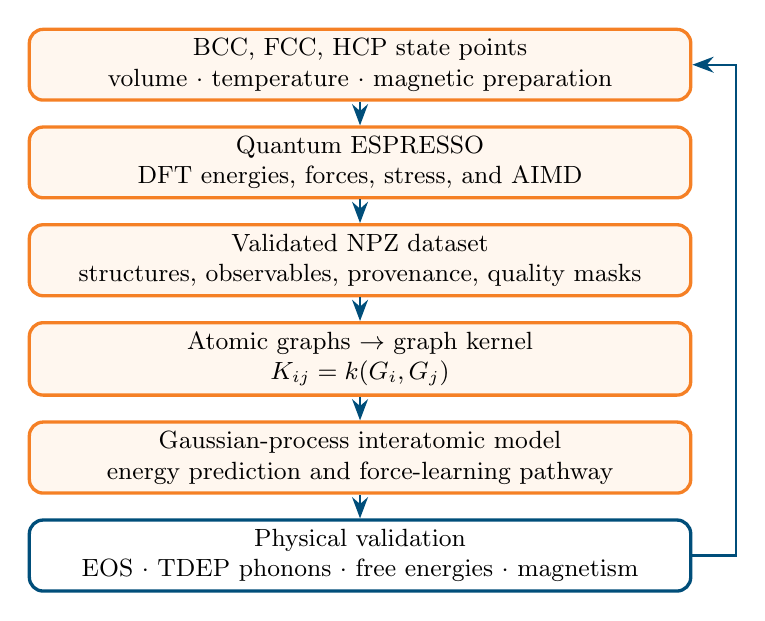
\begin{tikzpicture}[
  node distance=0.30cm,
  every node/.style={font=\small,align=center},
  process/.style={draw=uteporange,very thick,rounded corners=5pt,fill=utepsoft,minimum width=8.4cm,minimum height=0.82cm},
  validation/.style={draw=utepblue,very thick,rounded corners=5pt,fill=white,minimum width=8.4cm,minimum height=0.82cm},
  arrow/.style={-{Stealth[length=2.7mm]},thick,draw=utepblue}
]
\node[process] (states) {BCC, FCC, HCP state points\\volume $\cdot$ temperature $\cdot$ magnetic preparation};
\node[process,below=of states] (qe) {Quantum ESPRESSO\\DFT energies, forces, stress, and AIMD};
\node[process,below=of qe] (archive) {Validated NPZ dataset\\structures, observables, provenance, quality masks};
\node[process,below=of archive] (graphs) {Atomic graphs $\rightarrow$ graph kernel\\$K_{ij}=k(G_i,G_j)$};
\node[process,below=of graphs] (model) {Gaussian-process interatomic model\\energy prediction and force-learning pathway};
\node[validation,below=of model] (physics) {Physical validation\\EOS $\cdot$ TDEP phonons $\cdot$ free energies $\cdot$ magnetism};
\draw[arrow] (states)--(qe);
\draw[arrow] (qe)--(archive);
\draw[arrow] (archive)--(graphs);
\draw[arrow] (graphs)--(model);
\draw[arrow] (model)--(physics);
\draw[arrow] (physics.east) -- ++(0.55,0) |- (states.east);
\end{tikzpicture}
\end{center}
\vspace{-0.25em}
\justifying\small
Graph-based structural similarity connects first-principles trajectories across phase, compression, thermal disorder, and magnetic state. Model validation is performed against physical observables, not energy regression alone.
}

\headerbox{Results}{name=results,column=1,below=methodology,above=bottom}{
\begin{center}
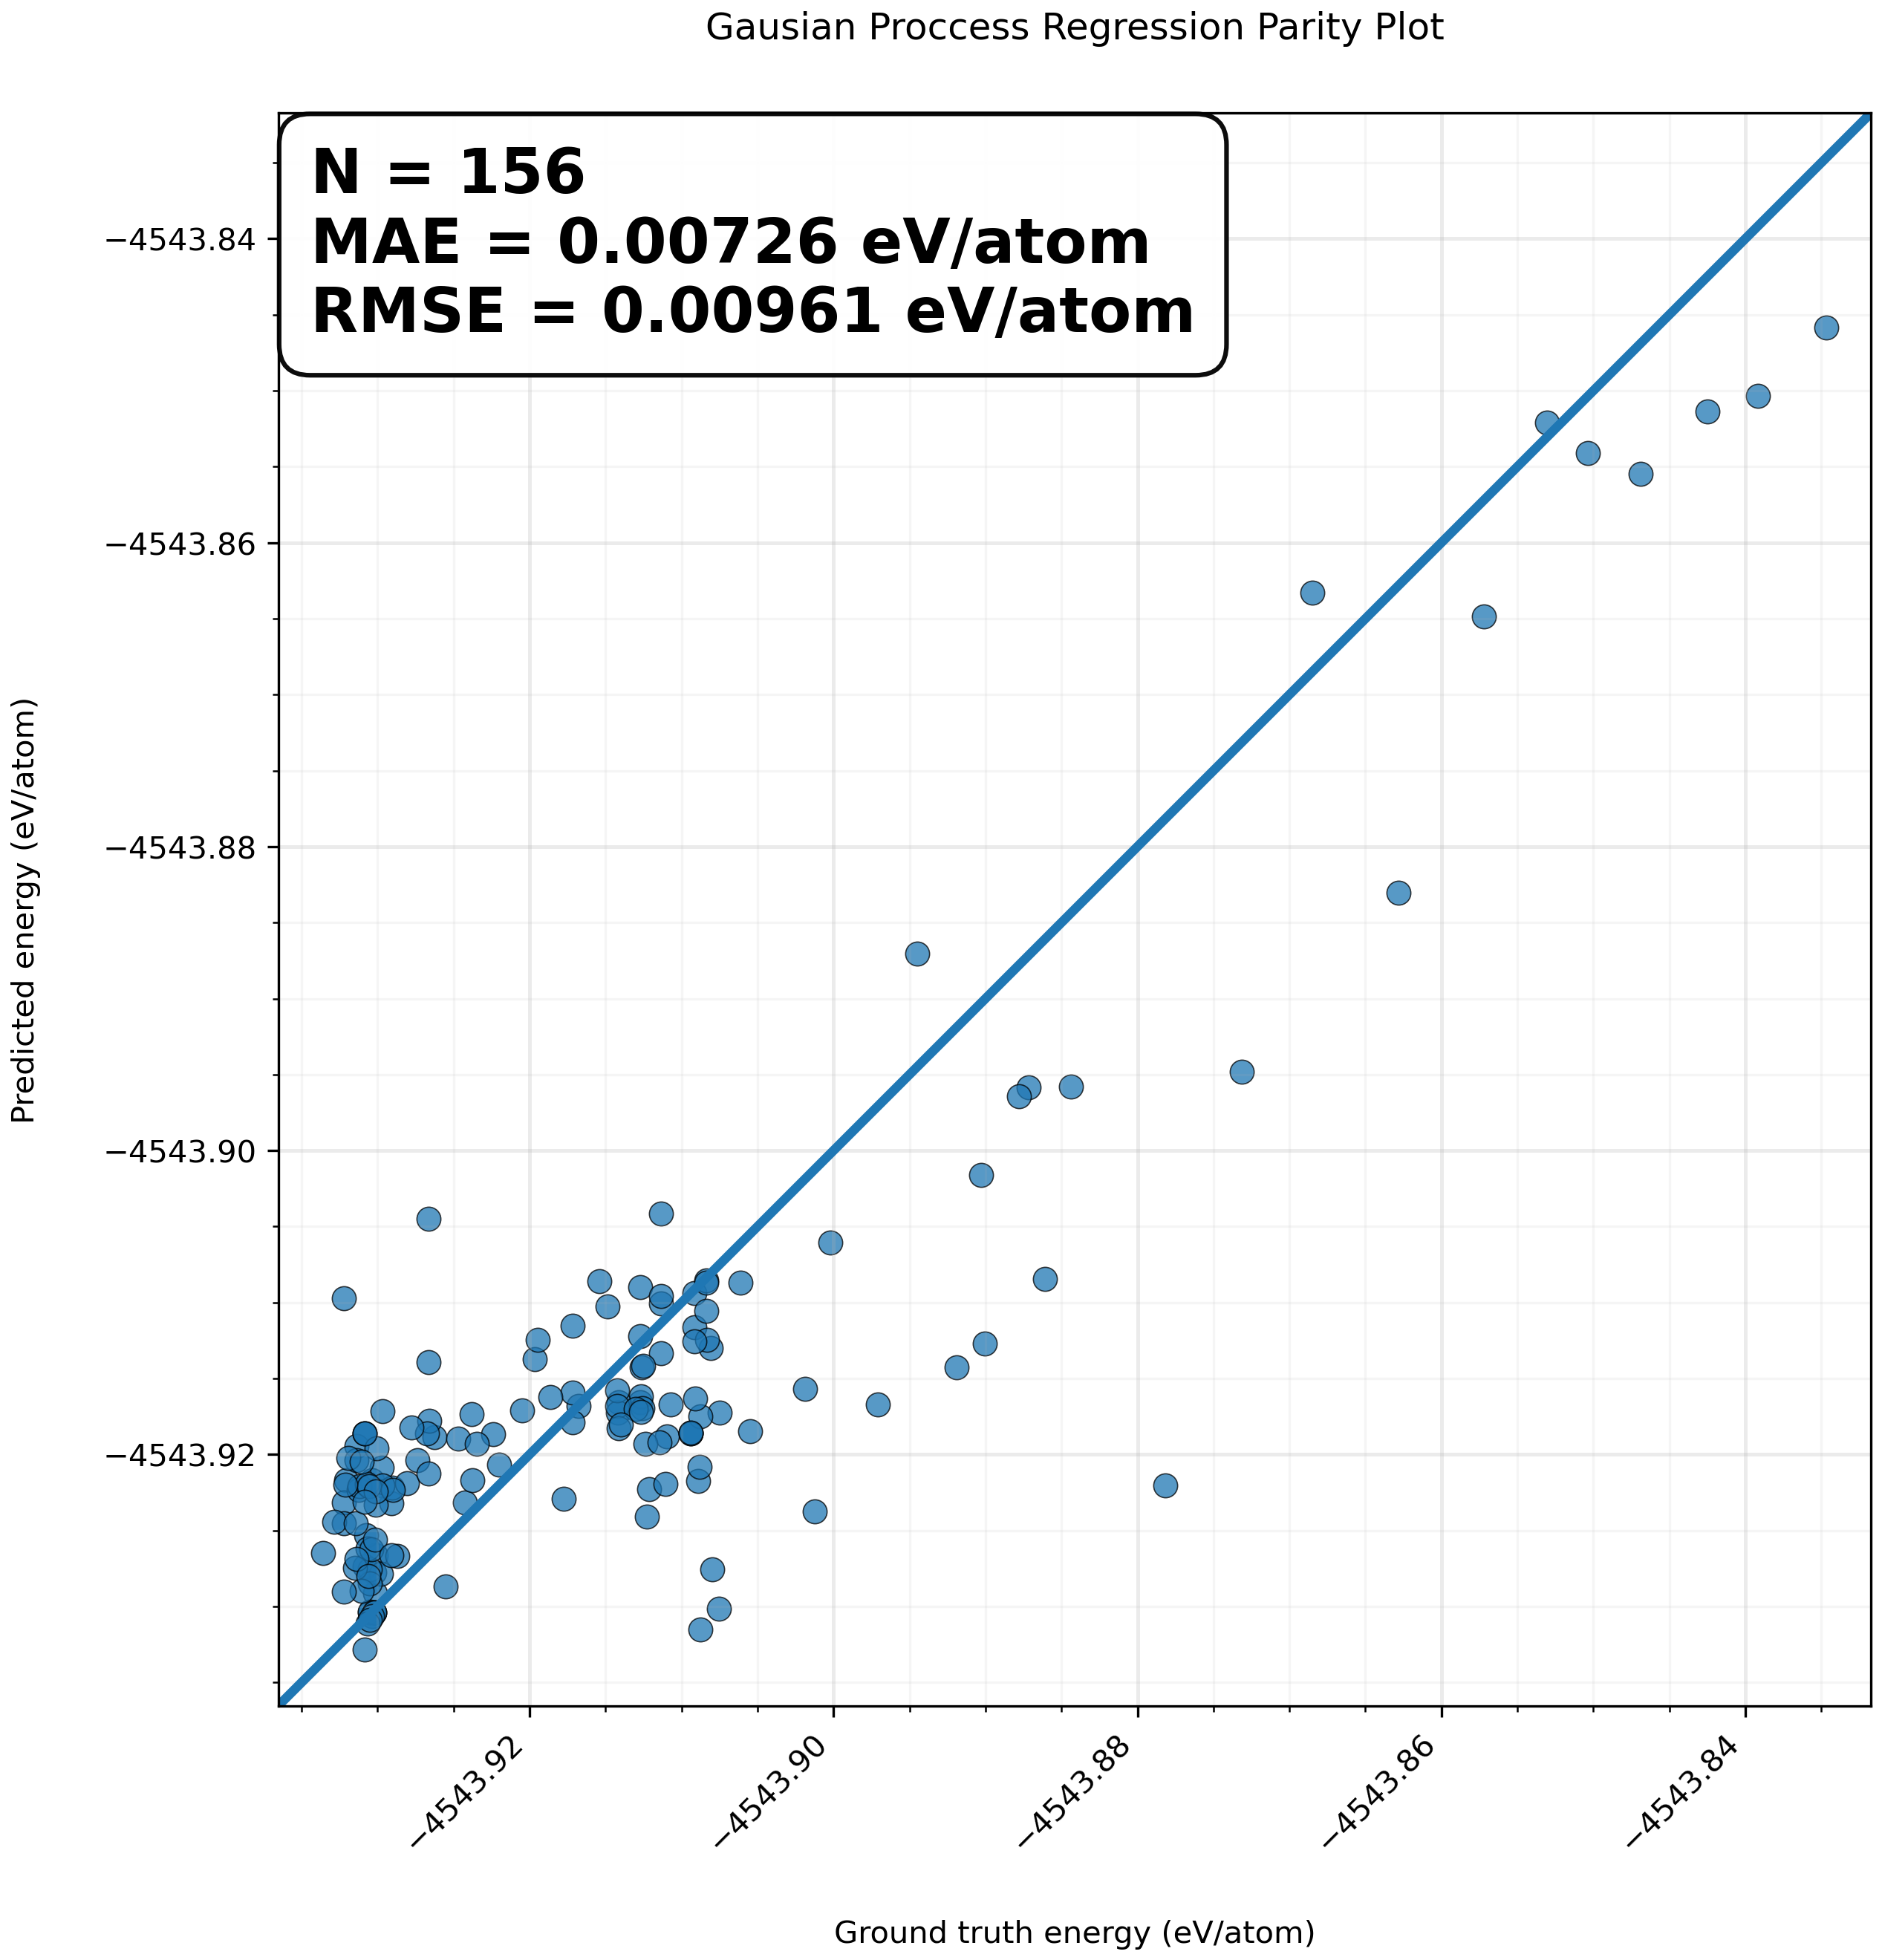
\includegraphics[width=0.92\linewidth]{figures/graph_kernel_parity.png}
\vspace{-0.45em}

\metric{7.26}{MAE (meV/atom)}\hfill
\metric{9.61}{RMSE (meV/atom)}\hfill
\metric{156}{evaluation structures}

\vspace{0.45em}
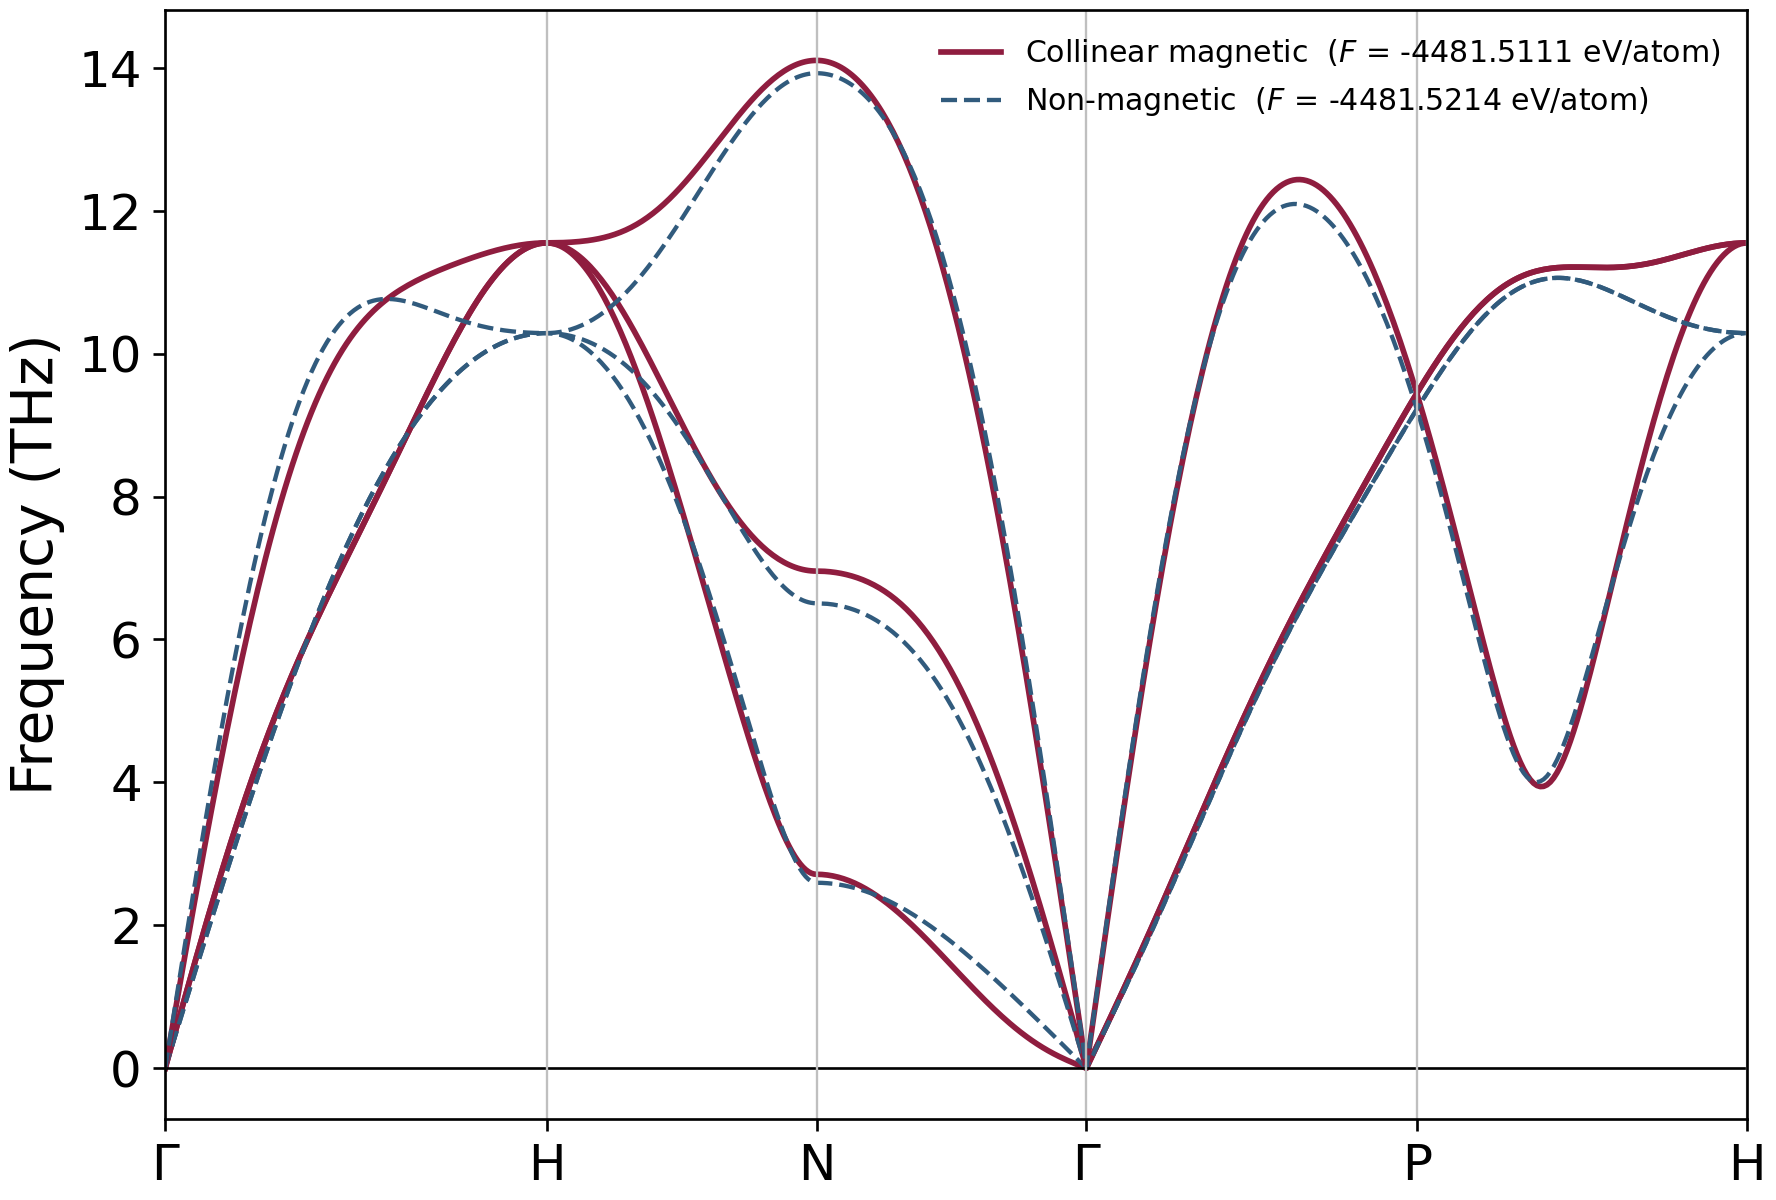
\includegraphics[width=0.98\linewidth]{figures/bcc_magnetic_phonons.png}
\end{center}
\vspace{-0.35em}
\small\justifying
The graph-kernel model reaches the 10 meV/atom scale. TDEP analysis finds dynamically stable magnetic and non-magnetic BCC phonons at 4000 K; the current magnetic fit uses 112 valid frames and remains a convergence-limited diagnostic rather than a final phase-stability result.
}

% ---------------------------------------------------------------------------
% COLUMN 3 — interpretation and closing material
% ---------------------------------------------------------------------------
\headerbox{Discussion}{name=discussion,column=2,row=0}{
\begin{itemize}\tightlist
  \item Graph kernels provide a flexible representation across structurally diverse iron phases.
  \item Energy accuracy is encouraging, but force, EOS, phonon, and free-energy validation remain essential.
  \item Magnetic preparation changes individual phonon branches and must be sampled systematically before drawing stability conclusions.
  \item The dataset now supports reproducible quality auditing at the trajectory and frame levels.
\end{itemize}
}

\headerbox{Future Work}{name=future,column=2,below=discussion}{
\begin{itemize}\tightlist
  \item train force components with trajectory-grouped splits;
  \item expand magnetic sampling across volume and temperature;
  \item compare BCC, FCC, and HCP free energies at matched conditions;
  \item benchmark scaling from direct DFT to thousand-atom ML simulations;
  \item release provenance, validation outputs, and reproducibility artifacts.
\end{itemize}
\vspace{0.35em}
\centering
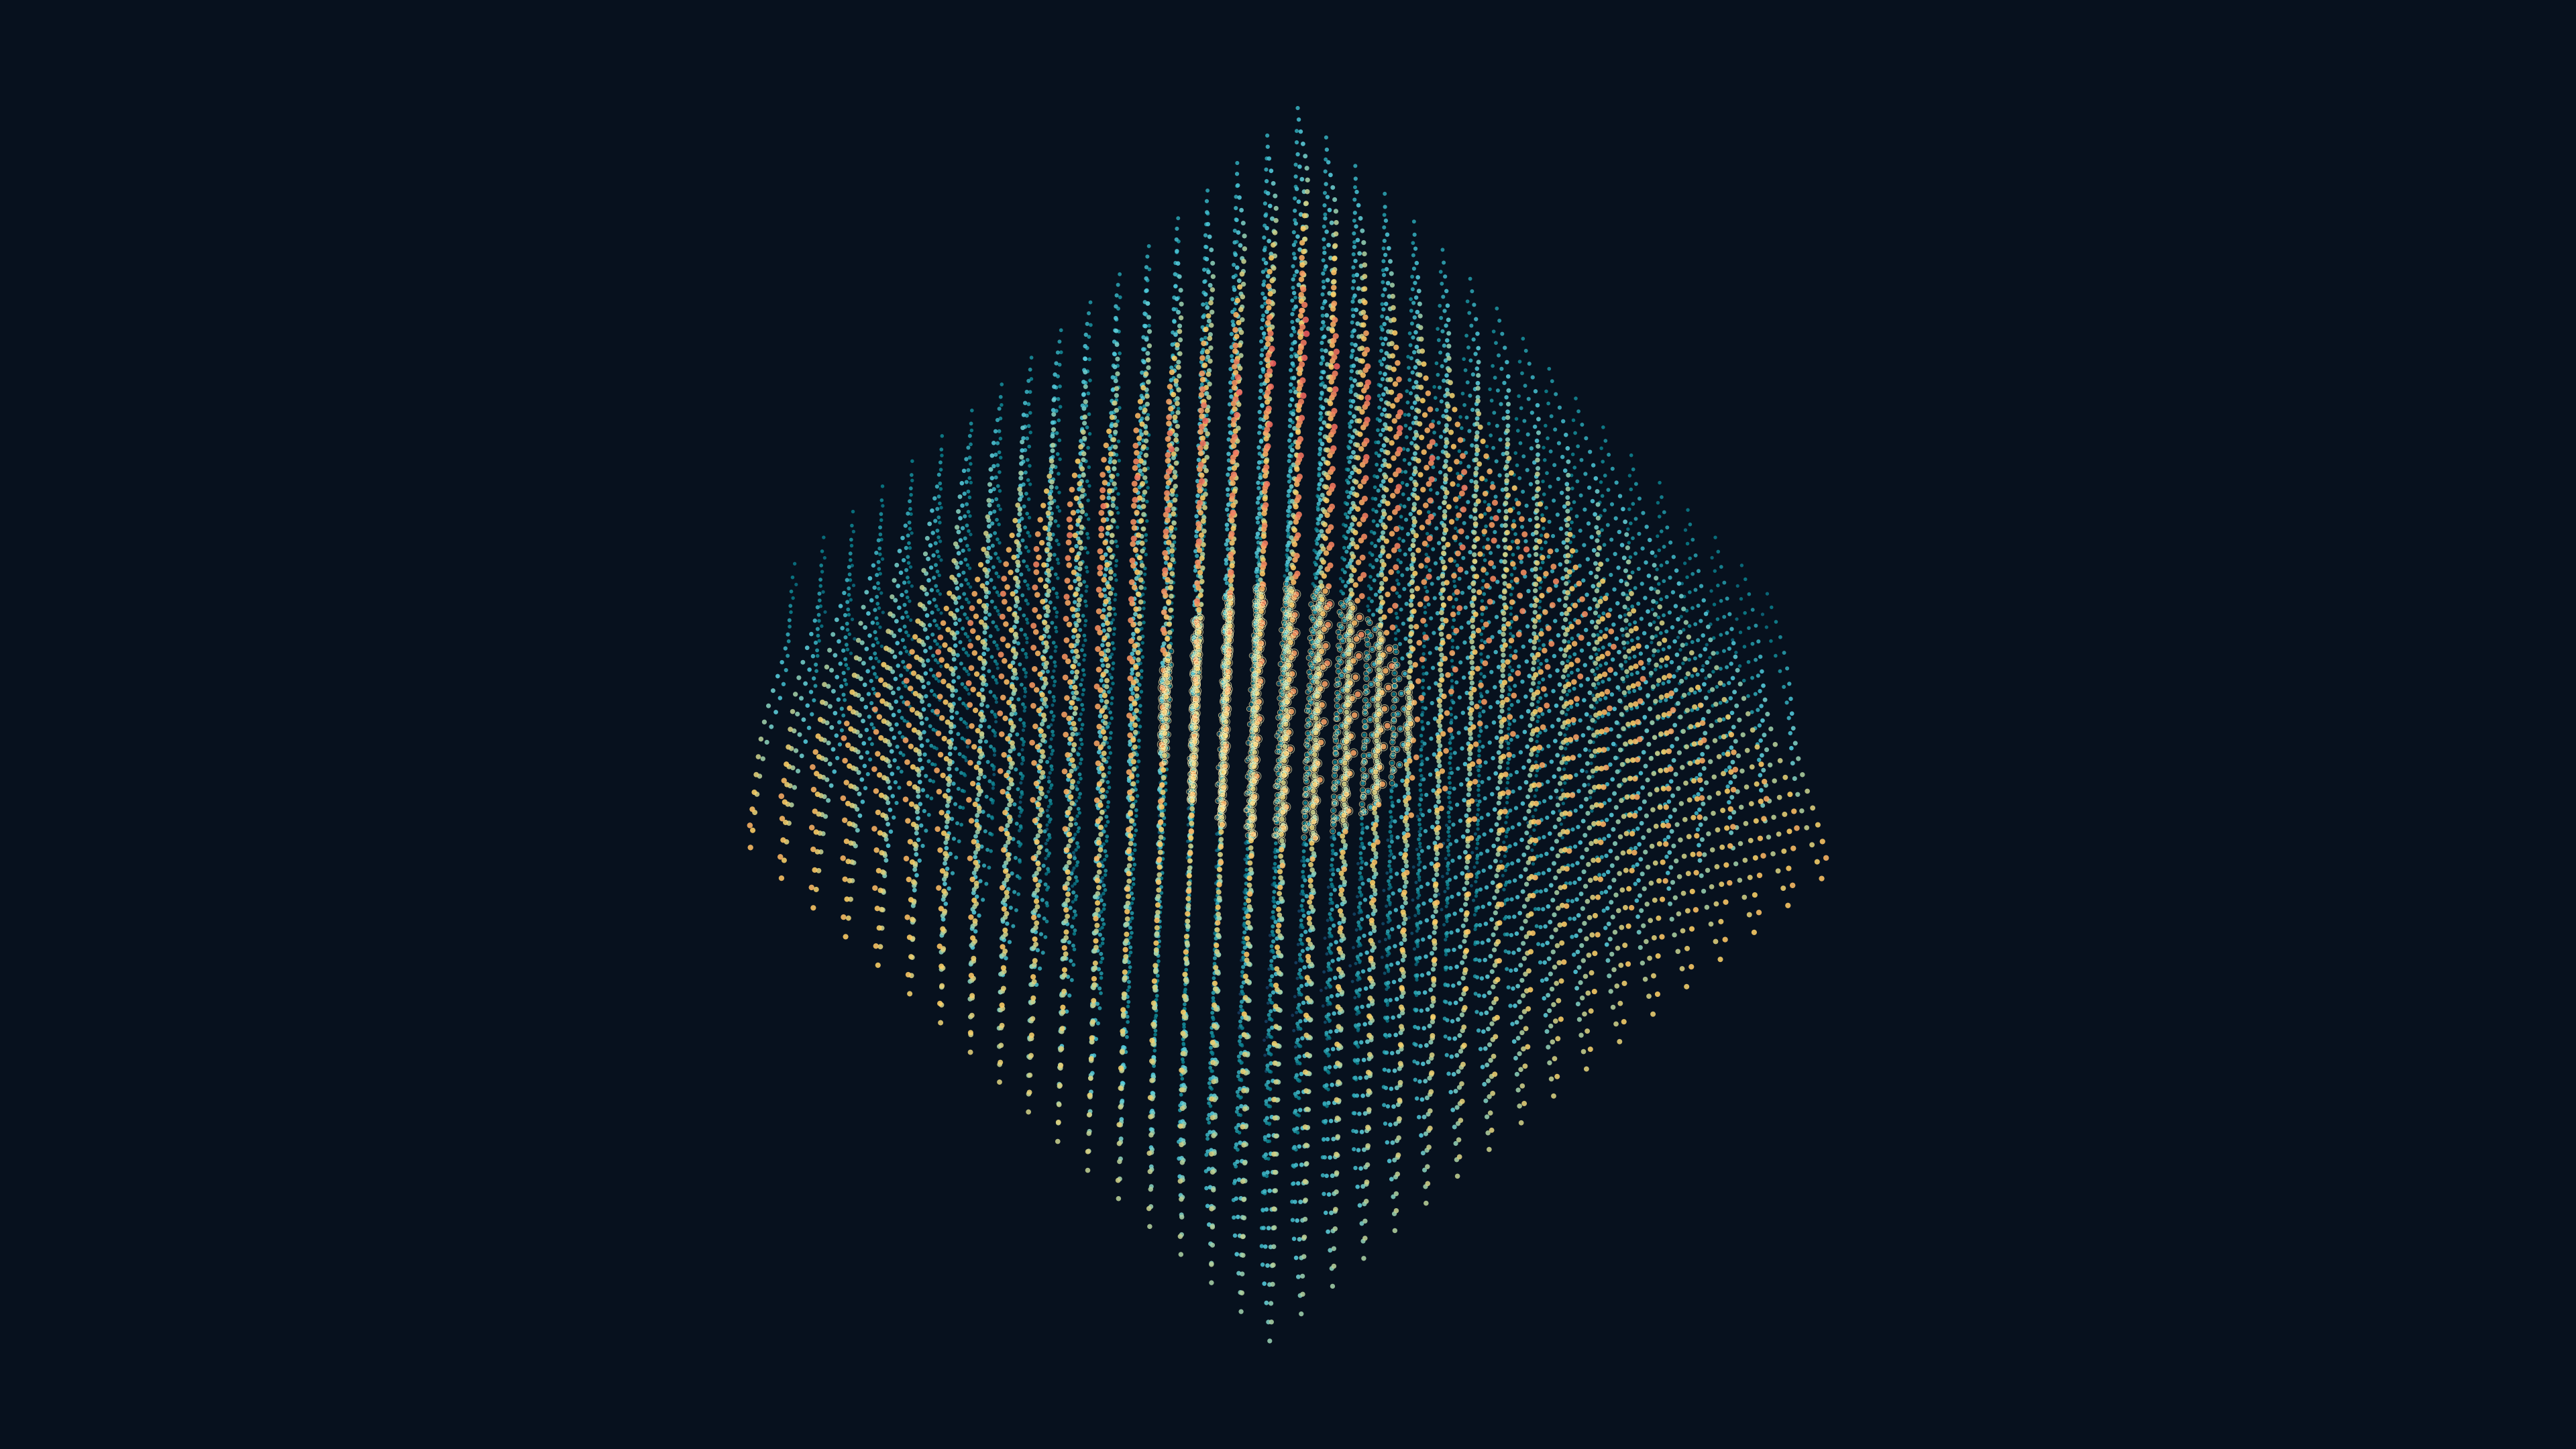
\includegraphics[width=0.90\linewidth]{figures/iron_ml_large_scale_simulation_space.png}
}

\headerbox{Acknowledgments}{name=ack,column=2,below=future}{
\small\justifying
Computational resources, collaborators, funding sources, and award numbers will be added before final submission.
}

\headerbox{References}{name=references,column=2,below=ack,above=bottom}{
\scriptsize\justifying
\begin{enumerate}[leftmargin=1.35em,itemsep=0.15em,topsep=0.1em]
  \item P. Giannozzi et al., ``QUANTUM ESPRESSO: a modular and open-source software project for quantum simulations of materials,'' \emph{J. Phys.: Condens. Matter} \textbf{21}, 395502 (2009).
  \item O. Hellman, I. A. Abrikosov, and S. I. Simak, ``Lattice dynamics of anharmonic solids from first principles,'' \emph{Phys. Rev. B} \textbf{84}, 180301 (2011).
  \item S. V. N. Vishwanathan et al., ``Graph kernels,'' \emph{J. Mach. Learn. Res.} \textbf{11}, 1201--1242 (2010).
  \item C. E. Rasmussen and C. K. I. Williams, \emph{Gaussian Processes for Machine Learning}, MIT Press (2006).
\end{enumerate}
}

\end{poster}
\end{document}
